% !TEX root = ../main.tex
\section{Approach}
\label{sec:approach}
In order to obtain reasonable and reliable pose of the fiducial tag under noisy condition, we fused the RGBD data of the Kinect One sensor. Our system first uses the depth sensor data to calculate an initial pose estimation of the detecting tag. Afterwards, we further refine the pose estimation by minimizing the reprojection error in RGB image using a constrained optimization method. In this section, we describe how we obtain the initial pose estimation of the tag using depth sensor data and fuse it with rgb information to refine the pose. Our key insight is that we can constrain the pose refinement process by weighting the sensor information with their uncertainty. In order words, we will weight the initial pose estimation more when the depth sensor is good otherwise we will allow the region of refinement to be bigger. 

\subsection{Depth Plane Fitting}
Since the fiducial tags are planar, we can obtain the pose the tag using depth sensor by fitting a plane over the depth points. Although the corners of the fiducial tags found in the RGB images might be noisy, they are accurate enough to locate the rough region of the tag with at most a few pixels of offset. With a calibrated RGBD sensor, we can extract the patch of depth points containing the planar tag. 

The raw range data retrieved from the Kinect One sensor are usually far from perfect for fitting an exact plane. Specifically, borders of the tag and some of the dark regions of the tag produce highly unreliable range data. Therefore, we first filter the data by removing points too far from the median before fitting the plane. Furthermore, the remaining points could have a large variance depending on the background lighting and the magnitude of the plane rotation. In the cases of depth sensor are noisy, we want to lower the weight of our initial pose estimate later in the pipeline. 

Therefore, we implemented a Bayesian plane fitting algorithm (describe the algorithm below) which assumes some noise model of the data and computes the mean and covariance of the plane. The noise model we used is a Kinect specific noise model [reference], which increases with the axis rotation of the depth plane. Note that a higher covariance implies that we are more uncertain about our fitting plane.

\begin{figure}
\centering
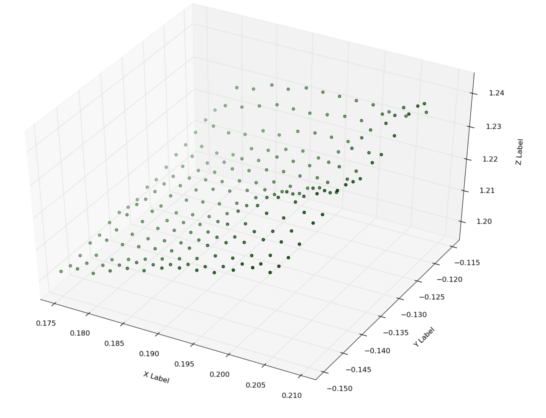
\includegraphics[width=\columnwidth]{figs/depth_plane_fig}
\caption{The fiducial tag plane captured by the depth sensor}
\label{fig:calib}
\end{figure}

\subsection{Initial Pose Estimation}
Once the plane is computed, we can estimate the pose of the tag. We project the noisy corners of the apriltag back onto the estimated plane to get their 3D coordinates in the camera frame. (Write out the formula) From here, the pose of the tag can be described as the homogenious transformation from the tag frame to the camera frame. We can solve for the transformation with a set of two 3D points correspondence: The 3D projected points of the tag in the camera frame and the 3D points in the tag frame. The points in the camera frame would be the projected corners which forms a $4X3$ matrix of homogeneous points denoted as $Pt_{obj}$. The points, $Pt_{tag}$ in the tag frame are the coordinate of the four corners measured from the center of the tag with depth of 0 because they are planar. 
$$Pt_{obj} = H Pt_{tag}$$
This becomes a 3-D rigid body transformation estimation problem. In our implementation:
\begin{align*}
p &= mean(Pt_{obj})\\
q &= mean(Pt_{tag})\\
x &=Pt_{obj} - p\\
y &=Pt_{tag} - q\\
U, S, V^T &= \textbf{SVD}(x^T y)\\
R &= VU^T \\
t &= q-Rp 
\end{align*}
$R$ and $t$ are the rotation and translation components of the the homogenous transform. When we projected the points onto the depth plane, the squares will likely deform. Therefore, we use the above algorithm to find the optimal transformation $H$ that minimizes the error in the least square sense. 
The pose obtained from the range data, although not always accurate, is rconsistent under noise and does not suffer from the perceptual ambiguity problem. 
\subsection{Pose Refinement}
Given the initial pose estimate of the tag and the RGB image, we can refine the pose that minimizes the reprojection error. Given camera model $K$, initial rotation and translation estimates $R_{init}$ and $t_{init}$
\begin{align*}
\hat{y} &= K[(R_{init} + \Delta R)x + (t_{init} + \Delta t)]\\
&\underset{\Delta R, \Delta t}{\mathrm{min}} (y - \hat{y})\\
&\text{subject to:} \\
& |\Delta R| <= \Gamma_R, \; |\Delta t| <= \Gamma_t\\
\end{align*}
The challenge here is to determine the region $\Gamma_R$ and $\Gamma_t$ which the initial pose estimate can be adjusted. If we unbound $\Delta R$ and $\Delta t$ the optimization, the solution might converge to a pose optimal for the reprojection error but far away from the true pose due to perceptual ambiguity. On the other hand, if we constrain the optimization too much, the final pose might not be far away from the true pose because of the inaccurate initial estimation. We recognize that the bound of on this optimization is related to the variance of the initial pose estimation. In one extreme, if there is no uncertainty in the depth camera and the range data are perfect, we don't need to further refine the pose of the tag. Similarly, if we don't have any depth information (uncertainty of the initial estimate is infinity), then the best we can do is find the pose solely based on the reprojection error which is the same as solving the unbounded optimization problem. Thererfore, this becomes a constrained optimization problem where the bound on the independent variables of $\Delta R$ and $\Delta t$ is proportional to the covariance of our estimated depth plane parameters. In our implementation, we used the trust-region algorithm to bound the optimization. The scaling threshold parameter is emperically tested to yield the best results for our robot. 